\documentclass[10pt]{article}
\usepackage{tikz}
\usetikzlibrary{shapes.misc}
\usepackage[margin=0cm]{geometry}
\pagestyle{empty}
\tikzstyle{every node}=[cross out, draw, red]

\begin{document}

\vspace*{\fill}
\begin{center}
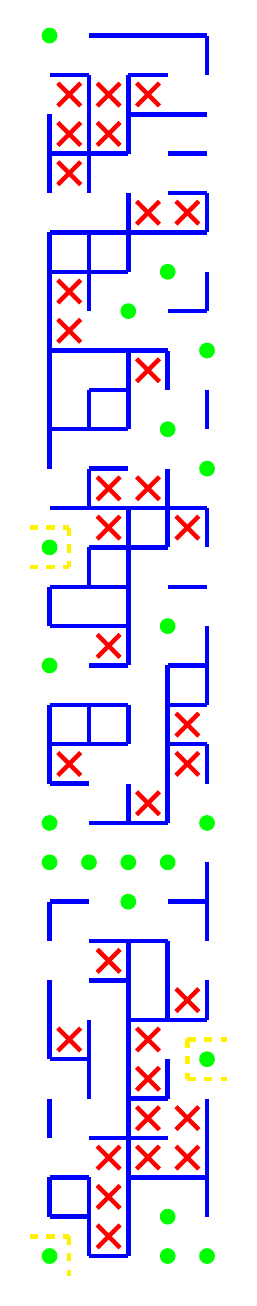
\begin{tikzpicture}[x=0.5cm, y=-0.5cm, ultra thick, blue]
% Walls
    \draw (1,0) -- (4,0);
    \draw (0,1) -- (1,1);
    \draw (2,1) -- (3,1);
    \draw (2,2) -- (4,2);
    \draw (0,3) -- (2,3);
    \draw (3,3) -- (4,3);
    \draw (3,4) -- (4,4);
    \draw (0,5) -- (4,5);
    \draw (0,6) -- (2,6);
    \draw (3,7) -- (4,7);
    \draw (0,8) -- (3,8);
    \draw (1,9) -- (2,9);
    \draw (0,10) -- (2,10);
    \draw (1,11) -- (2,11);
    \draw (0,12) -- (4,12);
    \draw (1,13) -- (3,13);
    \draw (0,14) -- (2,14);
    \draw (3,14) -- (4,14);
    \draw (0,15) -- (2,15);
    \draw (1,16) -- (2,16);
    \draw (3,16) -- (4,16);
    \draw (0,17) -- (2,17);
    \draw (3,17) -- (4,17);
    \draw (0,18) -- (2,18);
    \draw (3,18) -- (4,18);
    \draw (0,19) -- (1,19);
    \draw (1,20) -- (3,20);
    \draw (0,22) -- (1,22);
    \draw (3,22) -- (4,22);
    \draw (1,23) -- (3,23);
    \draw (1,24) -- (2,24);
    \draw (2,25) -- (4,25);
    \draw (0,26) -- (1,26);
    \draw (2,27) -- (3,27);
    \draw (1,28) -- (3,28);
    \draw (0,29) -- (1,29);
    \draw (2,29) -- (4,29);
    \draw (0,30) -- (1,30);
    \draw (1,31) -- (2,31);
    \draw (0,2) -- (0,4);
    \draw (0,5) -- (0,11);
    \draw (0,14) -- (0,15);
    \draw (0,17) -- (0,19);
    \draw (0,22) -- (0,23);
    \draw (0,24) -- (0,26);
    \draw (0,27) -- (0,28);
    \draw (0,29) -- (0,30);
    \draw (1,1) -- (1,4);
    \draw (1,5) -- (1,7);
    \draw (1,9) -- (1,10);
    \draw (1,11) -- (1,12);
    \draw (1,13) -- (1,14);
    \draw (1,17) -- (1,18);
    \draw (1,25) -- (1,27);
    \draw (1,29) -- (1,31);
    \draw (2,1) -- (2,3);
    \draw (2,4) -- (2,6);
    \draw (2,8) -- (2,10);
    \draw (2,12) -- (2,16);
    \draw (2,17) -- (2,18);
    \draw (2,19) -- (2,20);
    \draw (2,23) -- (2,31);
    \draw (3,8) -- (3,9);
    \draw (3,11) -- (3,13);
    \draw (3,16) -- (3,20);
    \draw (3,23) -- (3,25);
    \draw (3,26) -- (3,27);
    \draw (4,0) -- (4,1);
    \draw (4,4) -- (4,5);
    \draw (4,6) -- (4,7);
    \draw (4,9) -- (4,10);
    \draw (4,12) -- (4,13);
    \draw (4,15) -- (4,17);
    \draw (4,18) -- (4,19);
    \draw (4,21) -- (4,23);
    \draw (4,24) -- (4,25);
    \draw (4,27) -- (4,30);
% Pillars
    \fill[green] (0,0) circle(0.2);
    \fill[green] (3,6) circle(0.2);
    \fill[green] (2,7) circle(0.2);
    \fill[green] (4,8) circle(0.2);
    \fill[green] (3,10) circle(0.2);
    \fill[green] (4,11) circle(0.2);
    \fill[green] (0,13) circle(0.2);
    \fill[green] (3,15) circle(0.2);
    \fill[green] (0,16) circle(0.2);
    \fill[green] (0,20) circle(0.2);
    \fill[green] (4,20) circle(0.2);
    \fill[green] (0,21) circle(0.2);
    \fill[green] (1,21) circle(0.2);
    \fill[green] (2,21) circle(0.2);
    \fill[green] (3,21) circle(0.2);
    \fill[green] (2,22) circle(0.2);
    \fill[green] (4,26) circle(0.2);
    \fill[green] (3,30) circle(0.2);
    \fill[green] (0,31) circle(0.2);
    \fill[green] (3,31) circle(0.2);
    \fill[green] (4,31) circle(0.2);
% Inner points in accessible cul-de-sacs
    \node at (0.5,1.5) {};
    \node at (1.5,1.5) {};
    \node at (2.5,1.5) {};
    \node at (0.5,2.5) {};
    \node at (1.5,2.5) {};
    \node at (0.5,3.5) {};
    \node at (2.5,4.5) {};
    \node at (3.5,4.5) {};
    \node at (0.5,6.5) {};
    \node at (0.5,7.5) {};
    \node at (2.5,8.5) {};
    \node at (1.5,11.5) {};
    \node at (2.5,11.5) {};
    \node at (1.5,12.5) {};
    \node at (3.5,12.5) {};
    \node at (1.5,15.5) {};
    \node at (3.5,17.5) {};
    \node at (0.5,18.5) {};
    \node at (3.5,18.5) {};
    \node at (2.5,19.5) {};
    \node at (1.5,23.5) {};
    \node at (3.5,24.5) {};
    \node at (0.5,25.5) {};
    \node at (2.5,25.5) {};
    \node at (2.5,26.5) {};
    \node at (2.5,27.5) {};
    \node at (3.5,27.5) {};
    \node at (1.5,28.5) {};
    \node at (2.5,28.5) {};
    \node at (3.5,28.5) {};
    \node at (1.5,29.5) {};
    \node at (1.5,30.5) {};
% Entry-exit paths without intersections
    \draw[dashed, yellow] (-0.5,12.5) -- (0.5,12.5);
    \draw[dashed, yellow] (-0.5,13.5) -- (0.5,13.5);
    \draw[dashed, yellow] (3.5,25.5) -- (4.5,25.5);
    \draw[dashed, yellow] (3.5,26.5) -- (4.5,26.5);
    \draw[dashed, yellow] (-0.5,30.5) -- (0.5,30.5);
    \draw[dashed, yellow] (0.5,12.5) -- (0.5,13.5);
    \draw[dashed, yellow] (0.5,30.5) -- (0.5,31.5);
    \draw[dashed, yellow] (3.5,25.5) -- (3.5,26.5);
\end{tikzpicture}
\end{center}
\vspace*{\fill}

\end{document}
